\chapter{Spectral lines}
\section{Electron transitions and configurations}
The spectroscopic notation is a way to describe the energy levels of an atom or a molecule,
\begin{definition}[Spectroscopic notation]
\begin{equation}
  ^{\eqnmarkbox[blue]{S+1}{2S+1}}\eqnmarkbox[red]{L}{L}_{\eqnmarkbox[PineGreen]{J}{J}}^{\eqnmarkbox[orange]{p}{(p)}}.
\end{equation}
\annotate[yshift=-0.5em]{below, left}{S+1}{Spin multiplicity}
\annotate[yshift=-1.5em]{below, left}{L}{Orbital angular momentum}
\annotate[yshift=-0.5em]{below, right}{J}{Total angular momentum}
\annotate[yshift=1em]{above, right}{p}{Term parity}
\end{definition}
The parity characterizes whether the wave function changes sign under reflection of all electron positions through the origin. It is blank for even parity and $o$ for odd parity. The selection rules for the transitions are, 
\begin{itemize}
  \item Parity must change 
  \item $\Delta L = 0, \pm 1$ 
  \item $\Delta J = 0, \pm 1$, but $\Delta J = 0\rightarrow 0$ is forbidden
  \item Only one single electron wavefunction $n\ell$ can change with $\Delta\ell = \pm 1$ 
  \item $\Delta S = 0$ for electric dipole transitions
\end{itemize} 
This approximation is valid when radiation involved has $\lambda\gg a_0$.
Each electron is affected by the electric field produced by all other charges within the atom, 
\begin{equation}
  D_{ki} = \int \psi^*_k(\mathbf{r})\eqnmarkbox[red]{dipole}{\mathbf{D}}\psi_i(\mathbf{r})\,d\mathbf{r}.
\end{equation}
\annotate[yshift=-0.5em]{below, right}{dipole}{Dipole approximation}\\

\vspace{-5mm}
\textsf{Forbidden lines} are when one of the rules is not satisfied, while the \textsf{semi-forbidden lines} are where the spin selection rule is violated, and are much weaker than intersystem (permitted) transitions.
\subsection{Hydrogen transitions}
The different series of transitions are, 
\begin{itemize}
  \item \textsf{Lyman series} ($n=1$) in the UV
  \item \textsf{Balmer series} ($n=2$) in the visible
  \item \textsf{Paschen series} ($n=3$) in the IR
  \item \textsf{Brackett series} ($n=4$) in the far IR
  \item \textsf{Pfund series} ($n=5$) in the far IR 
\end{itemize}
The energy levels of hydrogen are given by the Rydberg formula, 
\begin{equation}
  E_n = -\frac{13.6\,\text{eV}}{n^2}. 
\end{equation} 

\begin{center}
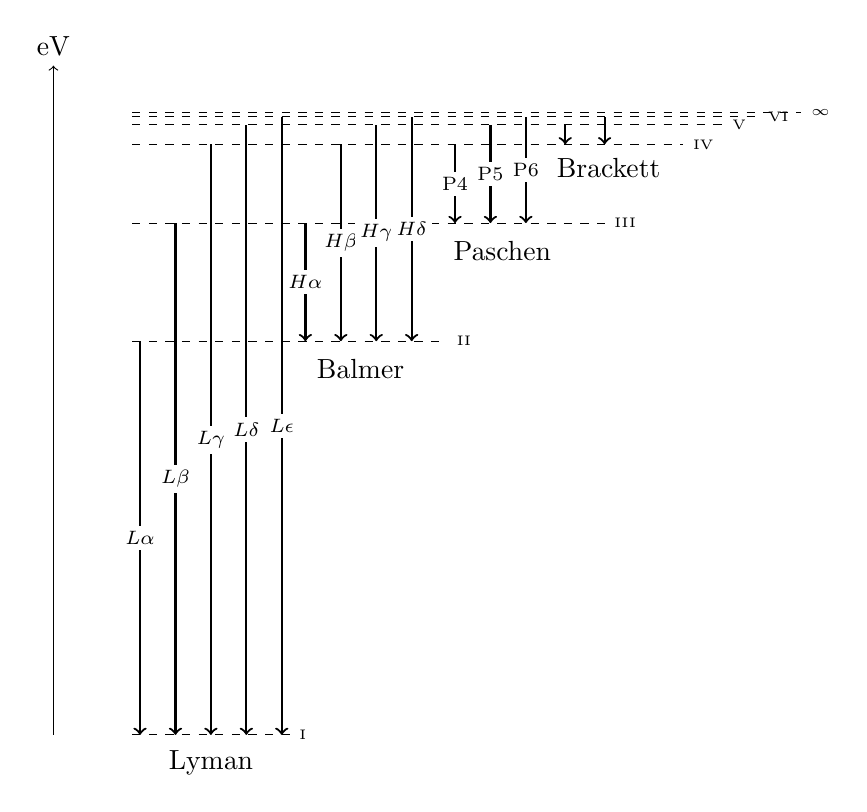
\begin{tikzpicture}
  \draw[->] (0,0) -- (0,8.5) node[above] {eV};
  %\draw[->] (-0.5,8) -- (10,8) node[right] {$n$};
  \draw[dashed] (1, 0) -- (3, 0) node[right] {\tiny{I}};
  \draw[dashed] (1, 5) -- (5, 5) node[right] {\tiny{II}};
  \draw[dashed] (1, 6.5) -- (7, 6.5) node[right] {\tiny{III}};
  \draw[dashed] (1, 7.5) -- (8, 7.5) node[right] {\tiny{IV}};
  \draw[dashed] (1, 7.75) -- (8.5, 7.75) node[right] {\tiny{V}};
  \draw[dashed] (1, 7.85) -- (9, 7.85) node[right, fill=white, inner sep=2pt] {\tiny{VI}};
  \draw[dashed] (1, 7.9) -- (9.5, 7.9) node[right] {\tiny{$\infty$}};

  \draw[thick, <-] (1.1, 0) -- (1.1, 5) node[midway, fill=white, inner sep=2pt] {\scriptsize{$\text{L}\alpha$}};
  \draw[thick, <-] (1.55, 0) -- (1.55, 6.5) node[midway, fill=white, inner sep=2pt] {\scriptsize{$\text{L}\beta$}};
  \draw[thick, <-] (2, 0) -- (2, 7.5) node[midway, fill=white, inner sep=2pt] {\scriptsize{$\text{L}\gamma$}};
  \draw[thick, <-] (2.45, 0) -- (2.45, 7.75) node[midway, fill=white, inner sep=2pt] {\scriptsize{$\text{L}\delta$}};
  \draw[thick, <-] (2.9, 0) -- (2.9, 7.85) node[midway, fill=white, inner sep=2pt] {\scriptsize{$\text{L}\epsilon$}};

  \draw[thick, <-] (3.2, 5) -- (3.2, 6.5) node[midway, fill=white, inner sep=2pt] {\scriptsize{$\text{H}\alpha$}};
  \draw[thick, <-] (3.65, 5) -- (3.65, 7.5) node[midway, fill=white, inner sep=2pt] {\scriptsize{$\text{H}\beta$}};
  \draw[thick, <-] (4.1, 5) -- (4.1, 7.75) node[midway, fill=white, inner sep=2pt] {\scriptsize{$\text{H}\gamma$}};
  \draw[thick, <-] (4.55, 5) -- (4.55, 7.85) node[midway, fill=white, inner sep=2pt] {\scriptsize{$\text{H}\delta$}};

  \draw[thick, <-] (5.1, 6.5) -- (5.1, 7.5) node[midway, fill=white, inner sep=2pt] {\scriptsize{P4}};
  \draw[thick, <-] (5.55, 6.5) -- (5.55, 7.75) node[midway, fill=white, inner sep=2pt] {\scriptsize{P5}};
  \draw[thick, <-] (6, 6.5) -- (6, 7.85) node[midway, fill=white, inner sep=2pt] {\scriptsize{P6}};

  \draw[thick, <-] (6.5, 7.5) -- (6.5, 7.75) node[midway] {};
  \draw[thick, <-] (7, 7.5) -- (7, 7.85) node[midway] {};

  \node at (2, -0.35) {Lyman};
  \node at (3.9, 4.65) {Balmer};
  \node at (5.7, 6.15) {Paschen};
  \node at (7.05, 7.2) {Brackett};

\end{tikzpicture}
\end{center}

\section{Line profiles}
The natural line profile is \textsf{Lorenzian},
\begin{equation}
  \phi(\nu) = \frac{1}{16\pi^2}\frac{4\eqnmarkbox[blue]{gamma}{\gamma_{ul}}}{(\nu-\eqnmarkbox[red]{nu}{\nu_{ul}})^2+\gamma_{ul}^2}, 
\end{equation}
\annotate[yshift=-0.5em]{below, right}{nu}{Frequency of the transition, $(E_u - E_l)/h$}
\annotate[yshift=1em]{above, right}{gamma}{Natural line width $\sum_{E_j < E_u}A_{uj} + \sum_{E_j < E_l}A_{lj}$}\\

\vspace{-5mm}
In addition to this, the \textsf{Voigt profile} is a convolution of the Lorenzian and Gaussian profiles,
\begin{Note}[Voigt profile]
\begin{equation}
  \phi(\nu) = \frac{1}{\sqrt{2\pi}} \int dv \frac{e^{-v^2/2\sigma^2}}{\sigma v} \frac{1}{16\pi^2}\frac{4\gamma_{ul}}{(\nu-(1-v/c)\nu_{ul})^2+\gamma_{ul}^2} 
\end{equation}
\end{Note}
which originates from the Doppler effect and the uncertainty principle.

\begin{center}
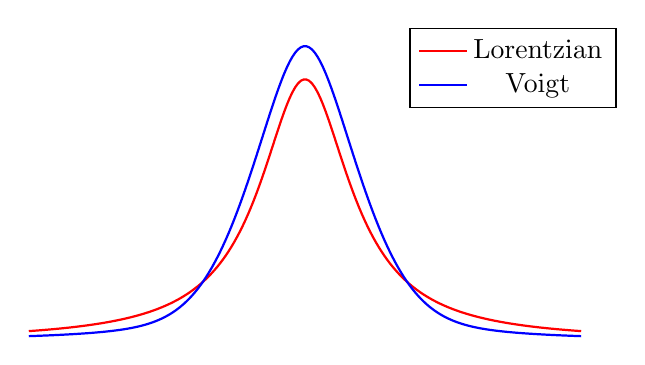
\begin{tikzpicture}
  \begin{axis}[
     hide axis,
      domain=-5:5,
      samples=200,
      xlabel={},
      ylabel={},
      width=10cm,
      height=6cm,
      legend pos=north east,
      title={},
  ]
    % Lorentzian profile: L(x) = 1/pi * (gamma)/(x^2 + gamma^2), here gamma=1.
    \addplot [red, thick] {1/pi * (1)/(x^2+1)};
    \addlegendentry{Lorentzian};
    % Pseudo-Voigt profile: V(x) = eta*L(x) + (1-eta)*G(x)
    % Gaussian: G(x) = 1/(sqrt{2*pi}) * exp(-x^2/2), here sigma=1.
    % eta = 0.5.
    \addplot [blue, thick] {0.5*(1/pi * (1)/(x^2+1)) + 0.5*(1/sqrt(2*pi))*exp(-x^2/2)};
    \addlegendentry{Voigt};
  \end{axis}
\end{tikzpicture}
\end{center}

\subsection{Equivalent width}
The spectral line \textsf{equivalent width} is defined as the area under the curve that is equivalent to the area of a rectangle of width $\Delta\lambda$ and height $I(\lambda)$,
\begin{equation}
  W_\lambda = \int \left(1-\frac{I(\lambda)}{I_c}\right)\,d\lambda. 
\end{equation}

\begin{center}
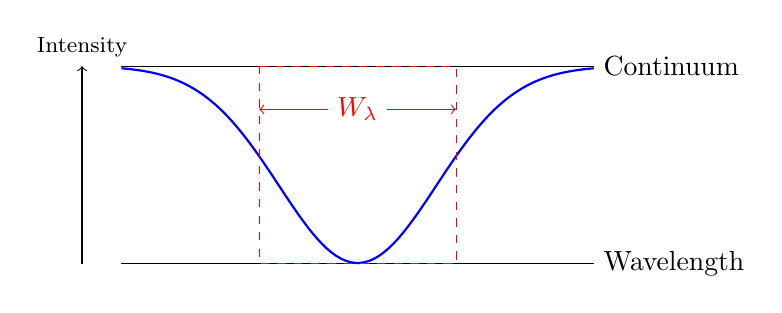
\begin{tikzpicture}[domain=-3:3, samples=100]
  % Draw the continuum line at y = 1.
  \draw (-3,1) -- (3,1) node[right] {Continuum};
  \draw (-3,-1.51) -- (3,-1.51) node[right] {Wavelength};
  % Draw the absorption feature (upside-down Gaussian).
  \draw[thick, blue] plot (\x, {1 - 2.5*exp(-(\x*\x)/2)});
  % Draw the dashed rectangle that represents the equivalent width.
  % The rectangle extends from x = -1.25 to 1.25 and from y = 0.5 to y = 1.
  \draw[red, dashed] (-1.25,1) rectangle (1.25,-1.51);
  
  % Draw an arrow below the rectangle to indicate the equivalent width.
  \draw[<->, red] (-1.25,0.45) -- (1.25,0.45) node[midway, fill=white] {$W_\lambda$};
  \draw[->] (-3.5, -1.51) -- (-3.5, 1) node[above] {\footnotesize{Intensity}};
  % Optionally, label the absorption feature.
  %\node[blue] at (0, {1 - 2.5*exp(0)}) [below] {Absorption};
\end{tikzpicture}
\end{center}

\subsection{Forbidden line notation}
Forbidden lines are transitions from metastable states and are written inside square brackets as,
\vspace{5mm}
\begin{equation}
  \eqnmarkbox[blue]{forb}{[}\eqnmarkbox[red]{O}{\text{O}}\eqnmarkbox[PineGreen]{III}{\text{III}}\eqnmarkbox[blue]{forb2}{]}
\end{equation}
\annotatetwo[yshift=1em]{above, left}{forb}{forb2}{Forbidden line}
\annotate[yshift=-0.5em]{below, left}{O}{Oxygen}
\annotate[yshift=-0.5em]{below, right}{III}{Doubly ionized state}\\

\section{Interstellar radiation fields}
The energetic photons can be divided into (most to least energetic),
\begin{itemize}
  \item \textsf{Synchotron radiation} -- galactic radiation from relativistic electrons in magnetic fields
  \item \textsf{CMB}
  \item \textsf{Starlight} -- UV photons from stellar photospheres
  \item \textsf{Mid and far IR emission} -- dust grains heated by starlight
  \item \textsf{Emission from plasma} -- at $T>10,000\,\text{K}$ -- free-free, free-bound, bound-bound, X rays
\end{itemize}

The ISM radiation fields determine the degree of ionization, gas and dust temperature and dynamics, and the dissociation degree of molecules.  
